\begin{song}{title=\centering Cestou do Jenkovic \\\normalsize Radůza  \vspace*{-0.3cm}}  %% sem se napíše jméno songu a autor
\moveright 3cm \vbox{      %Varianta č. 1  ---> Jeden sloupec zarovnaný na střed	

\sloka 
	^{D}Můj děda z kola ^{Hmi{\color{white}aaa}}seskočil, ^{C{\color{white}aa}}před prázdnou kašnou ^{A}na náměstí. 
	
	^{D}Na lavičce chleba ^{Hmi{\color{white}aaa}}posvačil, ^{C{\color{white}aaaa}}seřídil hodinky ^{A}na zápěstí.

\refren /: ^{D}A čápi z komína ^{A}od cihelny, zobákem ^{C{\color{white}aaaaa}}klapou, asi jsou ^{G{\color{white}aaaaaa}}nesmrtelný. :/

\sloka 
	Tři kluci v bílejch košilích dělili se o poslední spartu,

	ze zídky do záhonu skočili, přeběhli ulici a zmizeli v parku.

\refren 

\sloka 
	V oknech svítěj peřiny, na bílý kafe mlíko se vaří, 

	teď právě začaly prázdniny, venku je teplo a všechno se daří.

\refren



}
\setcounter{Slokočet}{0}
\end{song}


\begin{figure}[h]
\centering
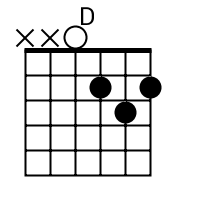
\includegraphics[width=3cm]{../Akordy/d.png}
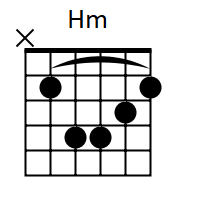
\includegraphics[width=3cm]{../Akordy/hm.png}
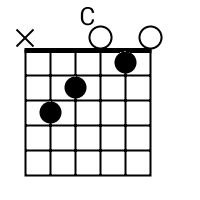
\includegraphics[width=3cm]{../Akordy/c.png}
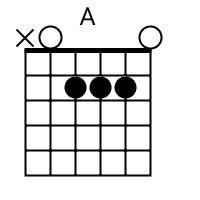
\includegraphics[width=3cm]{../Akordy/a.png}
\end{figure}
